\documentclass[14pt]{extarticle}
\usepackage[top=2.54cm, bottom=2.54cm, left=2.54cm, right=2.54cm]{geometry}
\usepackage{graphicx}
\usepackage[dvipsnames]{xcolor}
\usepackage[spanish,es-tabla]{babel}
\usepackage[T1]{fontenc}
\usepackage[utf8]{inputenc}
\usepackage{amsmath, amsfonts, amssymb}
\usepackage{physics, units}
\usepackage{listings}
\usepackage{enumerate}
\usepackage{apacite}
\decimalpoint
\usepackage{tikz}
\usetikzlibrary{calc}

\AtBeginDocument{\renewcommand\refname{Bibliografía}}
\newtheorem{theorem}{Teorema}[section]
\newtheorem{lemma}[theorem]{Lemma}
\newtheorem{proposition}[theorem]{Proposición}
\newtheorem{corollary}[theorem]{Corolario}

\newenvironment{proof}[1][Demostración]{\begin{trivlist}
		\item[\hskip \labelsep {\bfseries #1}]}{\end{trivlist}}
\newenvironment{definition}[1][Definición]{\begin{trivlist}
		\item[\hskip \labelsep {\bfseries #1}]}{\end{trivlist}}
\newenvironment{example}[1][Ejemplo]{\begin{trivlist}
		\item[\hskip \labelsep {\bfseries #1}]}{\end{trivlist}}
\newenvironment{remark}[1][Observación]{\begin{trivlist}
		\item[\hskip \labelsep {\bfseries #1}]}{\end{trivlist}}

\newcommand{\qed}{\nobreak \ifvmode \relax \else
	\ifdim\lastskip<1.5em \hskip-\lastskip
	\hskip1.5em plus0em minus0.5em \fi \nobreak
	\vrule height0.75em width0.5em depth0.25em\fi}

\definecolor{codegreen}{rgb}{0,0.6,0}
\definecolor{codegray}{rgb}{0.5,0.5,0.5}
\definecolor{commentgreen}{rgb}{0.1,0.6,0}
\definecolor{backcolour}{rgb}{0.96,0.96,0.96}

\lstdefinestyle{mystyle}{
	backgroundcolor=\color{backcolour},   
	commentstyle=\color{codegreen},
	keywordstyle=\color{cyan},
	numberstyle=\tiny\color{codegray},
	stringstyle=\color{commentgreen},
	basicstyle=\ttfamily\footnotesize,
	breakatwhitespace=false,         
	breaklines=true,                 
	captionpos=b,                    
	keepspaces=true,                 
	numbers=left,                    
	numbersep=5pt,                  
	showspaces=false,                
	showstringspaces=false,
	showtabs=false,                  
	tabsize=2
}

\lstset{style=mystyle}

\begin{document}

\begin{titlepage}

\begin{tikzpicture}[remember picture, overlay]
	\draw[line width = 4pt] ($(current page.north west) + (0.5in,-0.5in)$) rectangle ($(current page.south east) + (-0.5in,0.5in)$);
\end{tikzpicture}

\newcommand{\HRule}{\rule{\linewidth}{0.5 mm}} 

\center 

\begin{tabular}{llr}
	\hspace{-.95cm}\begin{minipage}{2cm}
		
\includegraphics[scale=0.33]{logo1.jpg}
	\end{minipage}
	& \hspace{0.2cm}
	\begin{minipage}{10cm}
		\begin{center}
		{\LARGE\textbf{\textsc{Universidad Nacional\\[-5pt] Autónoma de Honduras\\[5pt]}}}
		\end{center}
	\end{minipage}
	& %\hspace{-1cm}
	\begin{minipage}{2cm}
		
\includegraphics[scale=0.08]{logo2_001.jpg}	
	\end{minipage}
\end{tabular} \\[0.5cm]
 
\textsc{\Large \textbf{Facultad de Ciencias}}\\ 
\textsc{Escuela de Matemáticas y Ciencias de la Computación}\\[0.5cm]
\textsc{\small Carrera de Matemática}\\[2.cm]

\HRule \\[0.2cm]
{ \huge\bfseries Técnicas de Muestreo Espacial: Aplicaciones e Implementación en R\\[0.2cm] 
\HRule \\[3cm]}

\emph{Estudiante:}\\
\textsc{José Moisés Arias Núñez}\\
\textit{20141003876}\\[0.4cm]

\emph{Catedrático:}\\
\textsc{M. Sc. Roberto Duarte}\\[0.4cm]

{\emph{Presentado en:} Tegucigalpa, M.D.C. al\ \today}\\[0cm]

\end{titlepage}
\newpage
\tableofcontents

\newpage
\section*{Introducción}
\addcontentsline{toc}{section}{Introducción}

Los métodos estadísticos para el análisis de datos geográficamente distribuidos han probado ser gran importancia en temas de valor social y científico desde la segunda mitad de los años 80 y mostraron un crecimiento rápido en popularidad y desarrollo durante la década subsecuente. 

Las principales aplicaciones de importancia para estos métodos aparecen en el muestreo agrícola y forestal, pero también han mantenido su relevancia en la búsqueda de recursos energéticos fósiles y recursos minerales. El estudio de la contaminación ambiental y la predicción del clima se han visto fortalecidos gracias a la implementación del muestreo espacial como lo hacen notar \cite{Alinghaus.1996} y \cite{Hohn.1993}. 

Existe una variedad de metodologías utilizadas para el análisis de datos geográficos, pero tal vez la más popular en la literatura científica y académica es el \textit{kriging}. Esta técnica o, mejor dicho, colección de técnicas prueba ser sumamente versátil en la predicción de variables aleatorias espacialmente variadas. Posee diferentes versiones que se acoplan a distintas condiciones de variabilidad de los datos otorgando una reducción de la varianza en la predicción o estimación de la variable de interés. 

El método de \textit{kriging} o métodos de kriging surgen de un modelo básico de minimizar la varianza entre las observaciones regionales muestreadas y el predictor en la región de interés, bajo la condición de proveer un predictor insesgado. En este sentido, el mismo modelo del método ofrece una criterio para construir diseños muestrales. Pues tal como lo señala \cite{Cressie.1986} los resultados pueden ser independientes del uso de información muestral o datos de un pilotaje. 

La implementación de la estadística espacial está dotada de un arsenal bastante completo de métodos en \verb|R| para extraer variogramas y tendencias de los datos, así como representaciones visuales útiles de los datos recolectados en un experimento. Paquetes como \verb|geoR| cuentan con una documentación detallada en la comunidad en línea así como de textos diversos que ilustran la fortaleza de sus métodos. 

Este trabajo busca sintetizar los puntos más fuertes de estas técnicas y servir de punto de partida para llevar el estudio de la geoestadística a un nivel más profundo de comprensión y técnica. 


\newpage
\section*{Objetivos}
\addcontentsline{toc}{section}{Objetivos}
\begin{itemize}
	\item \textbf{Objetivo General}\\
	Ampliar los conocimientos sobre las técnicas de muestreo de una población en el contexto de unidades observacionales distribuidas en un espacio o región geográfica. 
	\item \textbf{Objetivos específicos}	
	\begin{enumerate}
		\item Integrar los modelos de muestreo básicos en el contexto de una muestra espacialmente variable. 
		\item Conocer las aplicaciones del muestreo espacial. 
		\item Implementar los métodos de muestreo espacial en R. 
	\end{enumerate}
\end{itemize}

\newpage
\section{Breve reseña histórica}
La aplicación de la estadística para recoger y analizar información sobre regiones geográficas ha cobrado una mayor importancia con el paso de los años. Instancias particulares de esto se dan en la agricultura\cite{Benedetti.2015}, la geología\cite{Thompson.2012}, la meteorología\cite{Cressie.1986} y la ecología\cite{Brus.2022}. 

De acuerdo con \cite{Alinghaus.1996}, las técnicas de muestreo espacial pueden rastrearse a fechas tan tempranas como las de la revolución industrial. El análisis de decaimiento a distancia, problemas en cartografía y biología datan desde inicios del siglo pasado, según la literatura científica resumida por \cite{Alinghaus.1996}. 

La importancia de los métodos de muestreo espacial va más allá de la academia, pues los estudios de este tipo permiten mejorar políticas sobre el manejo de recursos agrícolas y forestales\cite{Benedetti.2015}, predecir la existencia de recursos minerales y fósiles energéticamente explotables\cite{Thompson.2012, Cressie.1986, Journel.1987}, monitorear la distribución de especímenes en una región\cite{Brus.2022}, rastrear la propagación de una enfermedad o infección sobre los habitantes de una localidad, estimar la distribución de comunidades en una zona\cite{Benedetti.2015}, etc. 

A los métodos estadísticos empleados para la agricultura se les ha conocido globalmente como \textit{agricultura estadística} y aborda estadísticas sobre productos agrícolas, pesca, ganado, seguridad alimenticia y forestación\cite{Benedetti.2015}. Los métodos empleados en el estudio de los suelos y la búsqueda de recursos minerales y fósiles se conocen conjuntamente como \textit{geoestadística}\cite{Thompson.2012}.

En particular, la geoestadística fue desarrollada para analizar datos geológicos distribuidos en el espacio de un cuerpo mineral con la intención de predecir reservas minerales\cite{Cressie.1986}. Sus principales proponentes, de acuerdo con \cite{Cressie.1986}, habrían sido Matheron, Whittle y Gandin. 

El método que interesa en este ensayo es el conocido como \textit{kriging}, una técnica desarrollada por Matheron\cite{Benedetti.2015, Cressie.1986} nombrada así por su atribución a Krige\cite{Cressie.1986}. El término \textit{kriging} suele usarse en inglés como verbo o sustantivo, dependiendo del contexto. En este trabajo se referirá a \textit{kriging} como un sustantivo, que es el uso extendido que se le dio en la literatura académica angloparlante\cite{Cressie.1986, Journel.1987}.

En particular, el término de \textit{kriging} se asigna a la predicción espacial con modelos geoestadísticos, según \cite{Brus.2022}, donde un modelo geoestadístico es un modelo estadístico de la variación espacial de una variable de estudio. El \textit{kriging} busca una optimización del tamaño muestral o del patrón espacial de las ubicaciones muestrales\cite{Brus.2022}. 

%\newpage
\section{Predicción Espacial: Kriging}
De acuerdo con \cite{Thompson.2012} y \cite{Alinghaus.1996}, en el muestreo espacial se contemplan cantidades ambientales, ecológicas o geológicas como una variable aleatoria que denotaremos con $y_t$ para una región $t$, cuyos valores son recolectados en una extensión de $n$ regiones, $t_1, t_2, \cdots, t_n$. El fin del método kriging, acierta \cite{Benedetti.2015}, es predecir una variable aleatoria $y_0$ en una región vecina aun no muestreada.  

La motivación principal para abordar muestreos en unidades distribuidas en una región con métodos especiales, radica en el hecho de que la información geográficamente distribuida tiene características y peculiaridades para las cuales los modelos muestrales tradicionales son inadecuados, señala \cite{Benedetti.2015}. Los métodos espaciales en estadística fortalecen el análisis de la información geográfica sujeta a variación de observaciones dependientes\cite{Alinghaus.1996}. 

Las \textit{unidades espaciales} del estudio se definen sobre una partición finita del dominio en formas regulares o irregulares que contienen un número de unidades observacionales\cite{Thompson.2012}; de estas unidades espaciales, el investigador selecciona aleatoriamente las que conformarán su espacio muestral. 

Tal vez la razón más fuerte para proceder de esta manera en una investigación geográfico-estadística es el hecho que las poblaciones espacialmente distribuidas son, en sí mismas, muy difíciles de muestrear dado que su esparcimiento puede no ser regular o presentar conglomerados dentro del dominio de estudio\cite{Benedetti.2015}.

Debido a que la variable de interés $y_0$ es una variable aleatoria concerniente a una región más dentro de la población de zonas a estudiar, no se le llama al método kriging uno de \textit{estimación}, sino, propiamente de \textit{predicción}\cite{Thompson.2012}. 

El método, en este sentido, busca una solución óptima\cite{Brus.2022} a una serie de ecuaciones en términos de una función de covarianzas o un variograma (el cual es una varianza de diferencias)\cite{Thompson.2012}. 

Refiriéndonos a \cite{Thompson.2012}, ambos acercamientos prueban ser equivalentes cuando se conoce exactamente la función de covarianzas o el variograma. 

Siguiendo a \cite{Cressie.1986}, el método kriging posee dos variantes conocidas como \textit{kriging ordinario} y el \textit{kriging universal}; el primero se caracteriza porque el conocimiento del arrastre o función de media permite que el variograma estacionario pueda estimarse, mientras que en el segundo marco de trabajo, el variograma es conocido para estimar el arrastre. 

En \cite{Benedetti.2015} se señala la existencia de una versión adicional, el \textit{kriging simple}, el cual contempla un conocimiento exacto de la media y la varianza en cada región; no obstante, debido a sus altas restricciones prácticas se utiliza en raras ocasiones. 

Aunque existen muchas versiones del \textit{kriging}, la mayoría parte del siguiente modelo genérico en \cite{Brus.2022}

\begin{align}
	y_t =& \mu_t +\epsilon_t\\
	\epsilon_t \sim& \mathcal{N}(0, \sigma^2)\\
	Cov(\epsilon_t, \epsilon_t') =& C(h)
\end{align}
 
\noindent donde $y_t$ es la variable regionalizada en la ubicación $t$, $\mu_t$ es la media en la ubicación $t$, $\epsilon_t$ es el residual en la ubicación $t$ entendido como la diferencia entre la variable de estudio $y$ y su media $\mu_t$. La función $C(h)$ es la covarianza de los residuales entre dos localidades separadas por un vector de desplazamiento $h = t - t'$. 

Este modelo básico se discutirá a mayor extensión en las subsecuentes secciones. 
 
\subsection{Función de Covarianza Espacial}
Este acercamiento es tradicional en la estadística\cite{Thompson.2012}, no obstante el variograma se ha empleado extensamente en la geoestadística\cite{Cressie.1986, Thompson.2012, Brus.2022}. 

Siguiendo a \cite{Benedetti.2015} y en concordancia con \cite{Cressie.1986}, las variables aleatorias $y_t$ (también denotadas $y(\mathbf{z})$ por \cite{Benedetti.2015}) son observaciones del proceso estocástico real-valuado definido sobre un dominio $D$

\begin{equation}
	\left\lbrace y_t : t \in D \subset \mathbb{R}^d \right\rbrace\label{proceso}
\end{equation}

\noindent donde $D$ es un espacio de dimensión $d$ continuamente variado y que ha sido observado en una serie de puntos dados $t_1,\ t_2,\ \cdots,\ t_n$ (o $\mathbf{z}_1,\ \mathbf{z}_2,\ \cdots,\ \mathbf{z}_n$, en la notación de \cite{Benedetti.2015}). El índice $t$ es un vector y se utiliza como un índice sobre \textit{el espacio}\cite{Cressie.1986}. 

En las aplicaciones geológicas y ecológicas, los valores de la variable de interés en diferentes sitios suelen ser dependientes entre sí, más aún, los valores en regiones vecinas tienden a guardar una correlación, advierte \cite{Thompson.2012}. La medida de relación entre las variables $y_1$ y $y_2$ asociadas a los sitios $t_1$ y $t_2$ es la covarianza, ec. \ref{covarianza}: 

\begin{equation}
	Cov(y_1, y_2) = E\left[\left(y_1 - E(y_1)\right)\left(y_2 - E(y_2)\right)\right]\label{covarianza}
\end{equation}

Cuando la covarianza entre dos sitios depende solo de sus posiciones relativas, se emplea una \textit{función de covarianza} $C(h)$. De acuerdo con \cite{Thompson.2012}, podemos obtener esta medida de relación entre los \textit{$y$-valores} de cualesquiera dos sitios separados por $h$ con

\begin{equation}
	C(h) = Cov(y_{t+h}, y_t)\label{funcion_covarianza}
\end{equation}

\noindent donde $h$ es el vector de desplazamiento desde la región $t_1$ hacia la región $t_2$. Cuando la covarianza depende de la distancia, $d = \norm{h}$, mas no de la dirección entre los sitios, se dice que el proceso es \textit{isotrópico} y la función de covarianza se denota $C(d)$, \cite{Thompson.2012}. 

En su discusión sobre las propiedades de los sitios, \cite{Benedetti.2015} agrega que suponiendo que el proceso espacial tiene una media $\mu_t$ para cada región $t$ y que la varianza existe para todos los sitios $t$, dicho proceso se llama \textit{estrictamente estacionario} si para cualquier $n\geq 1$ número de sitios $\left\lbrace t_i \right\rbrace_{i=1}^n$ y cualquier $h$, la distribución de observaciones $\left\lbrace y_t \right\rbrace_{t=t_1}^{t_n}$ es la misma que $\left\lbrace y_{t + h} \right\rbrace_{t=t_1}^{t_n}$. 

Para \cite{Thompson.2012} un proceso se llama \textit{estacionario de segundo orden} cuando el valor esperado de la variable de las observaciones regionales es constante entre ubicaciones, pero la covarianza depende solo del vector de desplazamiento.

Un proceso se llama \textit{débilmente estacionario}, continua \cite{Benedetti.2015}, cuando la media es constante a través de los sitios $t$ y el proceso es isotrópico en el sentido de \cite{Thompson.2012}. 

\begin{proposition}
	Si el proceso $\left\lbrace y_t : t \in D \subset \mathcal{R}^d \right\rbrace$ es estrictamente estacionario, entonces es débilmente estacionario.
\end{proposition}

De acuerdo con \cite{Benedetti.2015}, un proceso en el que $y_t$ no sea débilmente estacionario puede presentar estacionalidad en los incrementos $y_t - y_{t+h}$. Entonces se dice que $y_t$ es \textit{intrínsecamente estacionario} si\footnote{Aunque la suposición de que el valor esperado de la variable de interés es constante en cada sitio es rara vez cierta, ya que, de acuerdo con \cite{Cressie.1986}, los datos rara vez presentan estacionalidad.} $\mu_t = \mu$ y

\begin{equation}
	Var\left[y_t - y_{t+h}\right] = 2\gamma(h)\label{variograma}
\end{equation}

\noindent donde $2\gamma(h)$ recibe el nombre de \textit{variograma}, mientras que $\gamma(h)$ solo se conoce como semivariograma\cite{Thompson.2012, Cressie.1986, Benedetti.2015}. 

\subsection{Predicción Lineal: Kriging}
En la predicción lineal, también conocida como \textit{kriging ordinario}\cite{Cressie.1986, Brus.2022} se busca predecir el valor de una variable aleatoria $y_0$ de interés en un sitio $t_0$ a partir de la información disponible de un proceso estocástico ec. \ref{proceso}\cite{Hohn.1993}. 

Utilizaremos la notación de \cite{Thompson.2012} para formular el procedimiento:
\begin{itemize}
	\item \textit{$y$-valor} observado en el iésimo sitio de la muestra de tamaño $n$: $y_i$
	\item iésimo sitio en la muestra de $n$ sitios: $t_i$
	\item covarianza entre \textit{$y$-valores} de un sitio $i$ y un sitio $j$: $Cov(y_i, y_j) = c_{ij}$
	\item varianza del \textit{$y$-valor} en el sitio $t_i$: $Var(y_i) = c_{ii}$	
\end{itemize}

El objetivo es encontrar una función $\hat{y}_0$ de los $n$ \textit{$y$-valores} observados insesgada para $y_0$

\begin{equation}
	E\left(\hat{y}_0\right) = E\left(y_0\right)\label{insesgadeza}
\end{equation}

\noindent que minimice el error cuadrado medio de la predicción dada por

\begin{equation}
	MSPE = E\left(y_0 - \hat{y}_0\right)^2\label{MSPE}
\end{equation}

Es importante notar, señala\cite{Thompson.2012}, que aunque el mejor estimador de $y_0$ es la esperanza condicional de $y_0$ dada las observaciones $y_1, \cdots, y_n$, esto es muy difícil de conseguir dado que se precisa una conocimiento exacto de la distribución conjunta de las variables aleatorias. 

Un criterio más práctico es hallar una función lineal de los \textit{$y$-valores} insesgada y que minimice ec. \ref{MSPE}. Tal proceso de optimización se concreta mediante multiplicadores de Lagrange\cite{Thompson.2012, Brus.2022}. 

Dado 

\begin{equation}
	\hat{y}_0 = \sum_{i=1}^{n} a_i y_i\label{blup}
\end{equation}

\noindent se quieren hallar valores $\left\lbrace a_i \right\rbrace_{i=1}^{n}$ que minimicen ec. \ref{MSPE} sujeto a ec. \ref{insesgadeza}. El problema se reescribe en forma matricial como:

\begin{equation}
	\mathbf{f} = \mathbf{G}^{-1}\mathbf{h}\label{ecuacion_predictiva}
\end{equation}

\noindent donde las matrices $\mathbf{f}_{n+1\times 1}$, $\mathbf{h}_{n+1\times 1}$ y $\mathbf{G}_{n+1\times n+1}$ son

\begin{eqnarray}
	\mathbf{f} = \begin{pmatrix}
	a_1 \\ a_2 \\ \vdots\\ a_n \\ m
	\end{pmatrix}, & \mathbf{h} = \begin{pmatrix}
	c_{10} \\ c_{20} \\ \vdots \\ c_{n0} \\ 1
	\end{pmatrix}, & \mathbf{G} = \begin{pmatrix}
	c_{11} & c_{12} & \cdots & c_{1n} & 1\\
	c_{21} & c_{22} & \cdots & c_{2n} & 1\\
	\vdots & \vdots & \ddots & \vdots & \vdots\\
	c_{n1} & c_{n2} & \cdots & c_{nn} & 1\\
	1 & 1 & \cdots & 1 & 1\\
	\end{pmatrix}
\end{eqnarray}

El método de \textit{kriging ordinario} consiste en estimar los pesos de \textit{kriging} $\left\lbrace a_i \right\rbrace_{i=1}^n$ y el multiplicador de Lagrange $m$\cite{Brus.2022, Thompson.2012}. En \cite{Thompson.2012}, el mejor predictor lineal insesgado\footnote{BLUP por sus siglas en inglés} $\hat{y}_0$ en ec. \ref{blup} se conoce como \textit{predictor de kriging}. Y la \textit{varianza de kriging} o \textit{MSPE} se define como

\begin{equation}
	MSPE = E\left(y_0 - \hat{y}_0\right)^2 = c_{00} - \sum_{i=1}^{n}a_i c_{i0} - m\label{MSPE_kriging}
\end{equation} 

Ya que la covarianza no se puede conocer exactamente, se utiliza un estimador desde los datos provenientes de la misma investigación o de una base de datos de estudios previos\cite{Thompson.2012}. Para un proceso estacionario e isotrópico la covarianza en sitios a $d$ unidades de distancia puede estimarse con una colección de $n_d$ pares de ubicaciones a tal distancia $d$ de separación de manera simple con

\begin{equation}
	\hat{C}(d) = \frac{1}{n_d} \sum \left(y_{t_i} - \overline{y}\right) \left(y_{t_j} - \overline{y}\right)\label{estimador_covarianza}
\end{equation}

\noindent donde la suma se efectúa sobre los pares de sitios a distancia $d$ de separación. Seguido puede emplearse un método de mínimos cuadrados no lineal para obtener una función de covarianza y estimar la covarianza a cualquier distancia\cite{Thompson.2012}. 

Pero no cualquier función puede usarse para modelar la semivarianza bajo isotropía, pues se debe asegurar que la varianza del predictor de kriging sea positiva\cite{Brus.2022}. En este sentido, dos modelos preferidos en la práctica son el exponencial y el esférico. 

\subsection{Variograma}
En el caso de un proceso estacionario de segundo orden, \cite{Thompson.2012} explica que la función de covarianza y el variograma contienen información equivalente en tanto que 

\begin{equation}
	\gamma (h) = c(0) - c(h) \label{semivariograma_segundo_orden}
\end{equation}

\noindent donde $c(0) = Var(y_t)$, la varianza de $y$ en un sitio $t$ arbitrario. 

De acuerdo con \cite{Cressie.1986}, el variograma es más general que la función de covarianza, pues este aún existe para algunos procesos que no cumplen estacionalidad de segundo orden. \cite{Cressie.1989} hace hincapié en que el valor del kriging en el análisis geoestadístico es mucho mayor de lo acreditado, en tanto que la clase de los problemas que que involucran variogramas contiene a la clase de problemas que emplean funciones de covarianza.

Un método relativamente simple de estimar el variograma en función de la distancia entre dos sitios está dado por \cite{Thompson.2012} como

\begin{equation}
	2\hat{\gamma}(d) = \frac{1}{n_d}\sum (y_{t_i} - y_{t_j})^2 \label{estimador_variograma}
\end{equation}

Este acercamiento es recomendado\cite{Thompson.2012} en tanto que ec. \ref{estimador_variograma} es insesgado, pero \ref{estimador_covarianza} no lo es. 

Las ecuaciones de predicción pueden reescribirse en función del variograma en condiciones similares bajo covarianza estimada. El objetivo es nuevamente predecir el valor de la variable de interés en una región nueva, $\hat{y}_0$ usando las $n$ observaciones de \textit{$y$-valores} de manera insesgada:

\begin{equation}
	E\left(\hat{y}_0\right) = E\left(y_0\right) \label{insesgadeza_variograma}
\end{equation}

\noindent minimizando el \textit{MSPE}

\begin{equation}
	MSPE = E\left(y_0 - \hat{y}_0\right)^2\label{MSPE_variograma}
\end{equation}

\noindent Escribiendo el estimador lineal como

\begin{equation}
	\hat{y}_0 = \sum_{i=1}^{n} a_i y_i\label{estimador_predictivo_variograma}
\end{equation}

\noindent el problema se traduce en encontrar valores $a_1,\ a_2,\ \cdots,\ a_n$ que minimicen la ec. \ref{MSPE_variograma} sujeto a la condición ec. \ref{insesgadeza_variograma}. La solución de \cite{Thompson.2012} viene dada en forma matricial:

\begin{equation}
	\mathbf{a} = \mathbf{\Gamma}^{-1} \gamma\label{ecuacion_predictiva_variograma}
\end{equation}

\noindent donde las matrices $\mathbf{a}_{n+1\times1}$, $\gamma_{n+1\times1}$ y $\mathbf{\Gamma}_{n+1\times n+1}$ están dadas abajo:

\begin{table}[h]
	\centering
	\begin{tabular}{ccc}
		$\mathbf{a} = \begin{pmatrix}
		a_1 \\ a_2 \\ \vdots\\ a_n \\ m^*
		\end{pmatrix}$, & $\gamma = \begin{pmatrix}
		\gamma_{10} \\ \gamma_{20} \\ \vdots \\ \gamma_{n0} \\ 1
		\end{pmatrix}$, & $\mathbf{\Gamma} = \begin{pmatrix}
		\gamma_{11} & \gamma_{12} & \cdots & \gamma_{1n} & 1 \\
		\gamma_{21} & \gamma_{22} & \cdots & \gamma_{2n} & 1 \\
		\vdots & \vdots & \ddots & \vdots & \vdots \\
		\gamma_{n1} & \gamma_{n2} & \cdots & \gamma_{nn} & 1 \\
		1 & 1 & \cdots & 1 & 0 
		\end{pmatrix}$
	\end{tabular}
\end{table}

Dentro de este contexto la predicción ec. \ref{ecuacion_predictiva_variograma} satisface el MSPE de la siguiente forma, ec. \ref{MSPE_variograma2}

\begin{equation}
	MSPE = E\left(y_0 - \hat{y}_0\right)^2 = \sum_{i=1}^{n}a_i\gamma_{i0} + m^*\label{MSPE_variograma2}
\end{equation}

Tal como se mencionó en la sección anterior, un modelo adecuado para las funciones de covarianza y variograma deben ser definidos positivos, de tal manera que se evite una varianza predictiva negativa\cite{Cressie.1986}. 

Para un modelo de \textit{kriging} condicionado a isotropía, \cite{Brus.2022} dicta los siguientes parámetros para un modelo esférico del semivariograma:

\begin{enumerate}
	\item \textit{Nugget} $c_0$: es la intersección del variograma con el eje $y$. 
	\item \textit{Partial sill} $c_1$: es la diferencia entre la máxima semivarianza y el \textit{nugget}. 
	\item \textit{Range} $\phi$: la distancia a la cual la semivarianza alcanza su máximo valor.
\end{enumerate}

Bajo estos criterios, se define el semivariograma esférico de la siguiente forma:

\begin{equation}
	\gamma (d) = \begin{cases}
	0 & \textrm{ si } d = 0 \\
	c_0 + c_1\left[1 - \frac{3}{2}\left(\frac{d}{\phi}\right) + \frac{1}{2} \left(\frac{d}{\phi}\right)\right] & \textrm{ si } 0 < d \leq \phi \\
	c_0 + c_1 & \textrm{ si } d > \phi
	\end{cases}
\end{equation}

\noindent Donde la suma $c_0 + c_1$ se conoce como \textit{varianza a priori}\cite{Brus.2022}. 

Por otro lado, un semivariograma exponencial con 3 parámetros, los mismos que \cite{Brus.2022} define para el caso esférico, presenta la siguiente forma

\begin{equation}
	\gamma(d) = \begin{cases}
	0 & \textrm{ si } d = 0\\
	c_0 + c_1 exp(-d/\phi) & \textrm{ si } d > 0
	\end{cases}
\end{equation}

Alternativamente, un modelo exponencial del variograma puede tomar una definición en el régimen no nulo como la utilizada por \cite{Hohn.1993}

$$\gamma(d) = c_1(1 - \exp(-d/\phi))$$

\noindent donde el modelo tiende asintóticamente hacia el \textit{sill}, con un acercamiento notable después de una distancia $d = 3\phi$. Además, \cite{Hohn.1993} propone un modelo de variograma completo que involucra una descomposición de $\gamma(h)$ en términos aditivos

$$\gamma(h) = \gamma_1(h) + \gamma_2(h) + \cdots + \gamma_n(h)$$

Tal marco de trabajo se conoce como \textit{modelos anidados} y son útiles en escenarios anisotrópicos donde la varianza presenta saturaciones en ciertas direcciones o los rangos varían según las direcciones entre sitios vecinos\cite{Hohn.1993}. 

\subsection{Predicción del Valor sobre una Región}
En muchas circunstancias se desea predecir el valor de la  media de la variable de interés sobre una región, cuando no su total\cite{Thompson.2012}. Las fórmulas discutidas en las secciones anteriores para realizar una predicción puntual $\hat{y}_0$ con su función de covarianza o variograma son válidas sobre una distribución discreta de la información\cite{Thompson.2012}; no obstante, pueden traducirse a un dominio continuo empleando integrales en su cómputo como lo muestran \cite{Cressie.1986}, \cite{Grondona.1991} y \cite{Thompson.2012}.  

Si $A$ es una región de estudio  particionada en $N$ sitios, \cite{Thompson.2012} y \cite{Grondona.1991} definen la predicción $y_0$ como

\begin{equation}
	y_0 = \frac{1}{\abs{A}} \int_{A} y_t \dd{t}
\end{equation}

\noindent suponiendo que el área de cada partición tiene el mismo valor $A$. La semivarianza media entre el iésimo sitio y la región $A$ está dado por:

\begin{equation}
	\gamma_{i0} = \frac{1}{\abs{A}} \int_{A}\gamma(y_i - y_t)\dd{t}
\end{equation}

EL \textit{MSPE} se obtiene mediante

\begin{equation}
	E\left(y_0 - \hat{y}_0\right)^2 = \sum_{i=1}^{n} a_i \gamma_{i0} + m^* - \gamma_{00}
\end{equation}

\noindent done la semivarianza media $\gamma_{00}$ está dada por

\begin{equation}
	\gamma_{00} = \frac{1}{N^2} \int_{A}\int_{A}\gamma(t-\nu)\dd{t}\dd{\nu}
\end{equation}

Un análisis de varianza es posible dentro de este contexto también, tal como lo demuestra \cite{Grondona.1991} en la aplicación al análisis de experimentos que toman en cuentan correlaciones espaciales entre los datos. 

Las estimaciones realizadas mediante bloques y aleatorización de las regiones muestrales prueban manejar de mejor manera las mediciones y ofrecen estimadores más eficientes, de acuerdo con \cite{Grondona.1991}. 

%\newpage
\section{Diseño espacial}
Siguiendo a \cite{Thompson.2012}, la función de covarianza o equivalentemente el variograma aportan suficiente información para establecer el número de sitios que se debe muestrear para hacer una predicción aceptable de la variable de interés en una nueva región. Según \cite{Cressie.1986}, incluso, los modelos de kriging permiten utilizar estudios piloto o bases de datos previas sobre una región para calibrar el instrumento de muestreo antes de realizar el kriging pertinente sobre la zona. 

En este sentido, un análisis del MSPE, bajo las condiciones básicas del kriging, provee una vía para elegir un tamaño muestral espacial $n$ idóneo para una predicción insesgada aceptable. De la expresión abajo

$$E\left(y_0 - \hat{y}_0\right)^2 = c_0 + \sum_{i=1}^{n}\sum_{i=1}^{n}a_i a_j c_{ij} -2 \sum_{i=1}^{n}a_i c_{i0}$$

\noindent se aprecia que las mejores predicciones resultan de las $n$ regiones muestra que tienen la menor covarianza entre sí, que es lo que sucede cuando se particiona la región de estudio en estratos pequeños\cite{Thompson.2012}, pero que poseen la mayor covarianza con el valor que se quiere predecir. 

Para variograma cuyas estimaciones de semivarianza decrecen con la distancia, se puede establecer que las regiones que más cerca están de la región de interés son los que mostrarán la mayor covarianza con respecto a dicha región de interés\cite{Thompson.2012}. 

%\newpage
\section{Implementación en R}
\subsection{Aplicación del \textit{kriging ordinario}}
\begin{example}[Ejemplo 1: Predicción por \textit{kriging ordinario}]
	Datos sobre estudios de camarones provenientes del \textit{Alaska Department of Fish and Game} en las proximidades de la Isla Kodiak, Alaska, fueron utilizados para estimar una función de covarianza espacial, la cual se empleó a su vez para predecir la cantidad de capturas en una nueva ubicación no muestreada previamente. Los datos de capturas fueron ploteados por ubicación en una tabla de la región de estudio registrando los pesos en libras ($\unit{lbs}$) y las distancias en millas náuticas ($\unit{nmi}$). Una unidad de investigación arrastró una línea de pesca por aproximadamente $\unit[1]{nmi}$ en un patrón grillado. Las covarianzas muestrales se obtuvieron usando pares de datos compactos en intervalos de distancias. Luego se ajustó los estimados de covarianza mediante mínimos cuadrados no lineales a una curva exponencial obteniendo la siguiente función de covarianza:
	
	\begin{equation*}
		C(x) = 5.1 \exp(-0.49x)
	\end{equation*}
	
	Supóngase que una de las grúas atrapó $y_1 = \unit[5.526]{klbs}$ y una segunda grúa consiguió capturar $y_2 = \unit[1.417]{klbs}$ a $\unit[6]{nmi}$ de distancia. ¿Cuál puede ser el tamaño (en libras) de una captura a $\unit[1]{nmi}$ de la primera captura y $\unit[5.4]{nmi}$ de la segunda?
\end{example}\label{ejemplo1_camarones}

\paragraph{Solución}
La varianza es $C(0) = 5.1$. La covarianza entre las grúas a $\unit[6]{nmi}$ de separación es $c_{12} = 5.1\cdot \exp(-0.49\cdot 6) = 0.3$. Mientras que las covarianzas con respecto al nuevo sitio $t_0$ son $c_{10} = 3.1$ y $c_{20} = 0.4$, respectivamente para el sitio 1 y el sitio 2. La ecuación predictiva \ref{ecuacion_predictiva} toma la forma definida:

\begin{align*}
	\begin{pmatrix}
	a_1 \\ a_2 \\ m 
	\end{pmatrix} = \begin{pmatrix}
	5.1 & 0.3 & 1 \\
	0.3 & 5.1 & 1 \\
	1 & 1 & 0 \\
	\end{pmatrix}^{-1} \begin{pmatrix}
	3.1 \\ 0.4 \\ 1
	\end{pmatrix}
\end{align*}

El siguiente script de \verb|R| computa el resultado con valores $a_1 = 0.78$, $a_2 = 0.22$ y $m = -0.95$ para un \textit{BLUP}, ec. \ref{blup}, de $\hat{y}_0 = \unit[4.622]{klbs} = \unit[4622]{lbs}$. El \textit{MSPE}, ec. \ref{MSPE_kriging}, es de $3.5$ para un error cuadrático medio, \textit{MSE}, de $\unit[1.9]{klbs} = \unit[1900]{lbs}$.

\lstinputlisting[language = R, caption = Ejemplo de predicción mediante kriging ordinario, label = ejemplo_camarones_alaska]{proyecto_kriging/ejemplo_camarones.R}

\subsection{Cómputo del variograma}

\begin{example}[Ejemplo 2: Re-evaluado mediante \textit{semivariograma}]
	Este ejemplo se desarrolla sobre el enunciado del ejemplo \ref{ejemplo1_camarones}, esta ves incorporando el cálculo del semivariograma calculado a partir de la ec. \ref{semivariograma_segundo_orden}. 
	
	$$\gamma(x) = 5.1 - 5.1 \exp(-0.49 x)$$
\end{example}

\paragraph{Solución}
La semivarianza para las grúas a $\unit[6]{nmi}$ de distancia es

$$\gamma_{12} = 5.1(1 - \exp(-0.49\cdot6)) = 4.8$$

Las semivarianzas con respecto al nuevo sitio son $\gamma_{10} = 2.0$ y $\gamma_{20} = 4.7$, respectivamente para la grúa en la ubicación $t_1$ y la grúa en la ubicación $t_2$. La ecuación predictiva, ec. \ref{ecuacion_predictiva_variograma}, cobra la forma

\begin{equation}
	\begin{pmatrix}
	a_1 \\ a_2 \\ m^*
	\end{pmatrix} = \begin{pmatrix}
	0 & 4.8 & 1 \\
	4.8 & 0 & 1 \\
	1 & 1 & 0
	\end{pmatrix}^{-1} \begin{pmatrix}
	2.0 \\ 4.7 \\ 1
	\end{pmatrix}
\end{equation} 

El siguiente script de \verb|R| computa el resultado con valores $a_1 = 0.78$, $a_2 = 0.22$ y $m^* = 0.95$ para un \textit{BLUP}, ec. \ref{blup}, de $\hat{y}_0 = \unit[4.622]{klbs} = \unit[4622]{lbs}$. El \textit{MSPE}, ec. \ref{MSPE_variograma2}, es de $3.5$ para un error cuadrático medio, \textit{MSE}, de $\unit[1.9]{klbs} = \unit[1900]{lbs}$.

\lstinputlisting[language = R, caption = Ejemplo de predicción mediante cómputo de variograma, label = ejemplo_camarones_alaska_variograma]{proyecto_kriging/ejemplo_camarones_variograma.R}

El paquete básico de \verb|R| para analizar datos geoestadísticos es \verb|geoR|. El ejemplo siguiente utiliza datos sobre una producción de frijol de soja disponibles en la librería \verb|geoR|. 

\lstinputlisting[language = R, caption = Ejemplo usando geoR, label = codigo_implementacion_geoR]{proyecto_kriging/ejemplo1_geoR.R}

La ejecución del código en listing \ref{codigo_implementacion_geoR} genera la gráfica en la figura \ref{variograma_geoR} que muestra los valores de semivarianza correspondientes a cada distancia a la cual se recogen las muestras. La línea de tendencia ayuda a determinar la forma particular de la función de semivarianza que debe implementarse para realizar las predicciones. 

\begin{figure}[h]
	\centering
	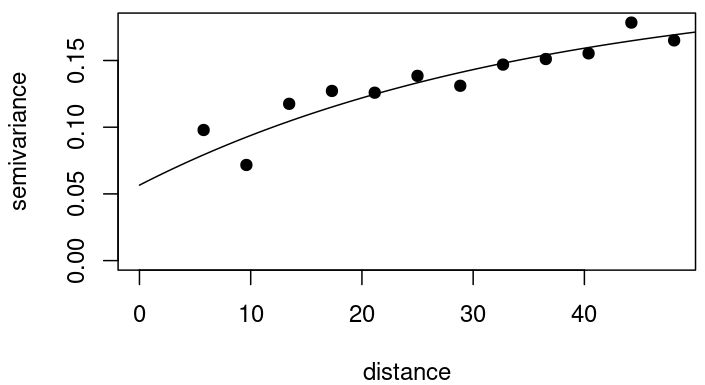
\includegraphics[scale=0.8]{proyecto_kriging/Rplot_variograma_ejemplo1.png}\caption{Gráfico de semivarianza contra distancia de los datos de producción de frijol de soja en listing \ref{codigo_implementacion_geoR}.}\label{variograma_geoR}
\end{figure}

En particular, para la ejecución de listing \ref{codigo_implementacion_geoR} la curva que mejor se ajusta (por mínimos cuadrados) a la distribución de puntos es una exponencial con \textit{Range} $\phi = 35.5832$, \textit{partial sill} $c_1 = 0.1520$ y \textit{nugget} $c_0 = 0.0566$. Estos datos pueden ser visualizados con el comando \verb|summary(fitted)|. 

Mediante el paquete \verb|geoR| es posible generar un mapa de contornos de la región muestreada, tal como se muestra en listing \ref{codigo_implementacion_geoR2}. 

\lstinputlisting[language = R, caption = Script para generar un mapa de contornos en R, label = codigo_implementacion_geoR2]{proyecto_kriging/ejemplo1_geoR2.R}

La figura \ref{mapa_contorno_geoR} muestra la distribución de las localidades muestreadas un cultivo de frijol de soja generada por \verb|R|. Se puede apreciar el mapa de contornos marcando delimitadores para las regiones de interés. 

\begin{figure}[h]
	\centering
	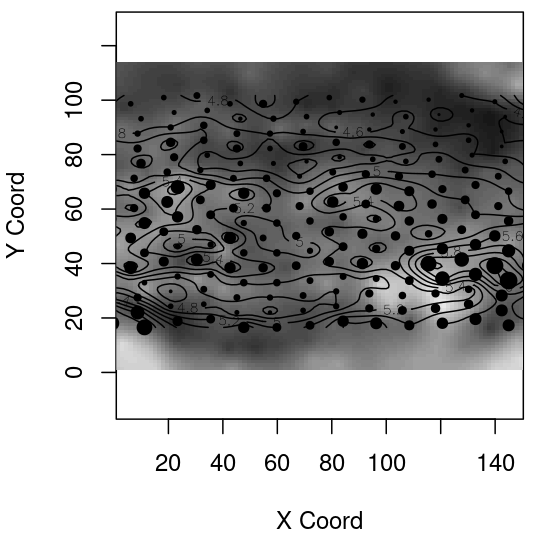
\includegraphics[scale=1.0]{proyecto_kriging/Rplot_mapa_contorno.png}\caption{Mapa de contorno de los datos muestreados en el código en listing \ref{codigo_implementacion_geoR2}.}\label{mapa_contorno_geoR}
\end{figure}

Existen formas de estimar el variograma utilizando el método de momentos y máxima verosimilitud sobre una base de datos geoespaciales, como lo explica extensamente \cite{Brus.2022}. Los paquetes \verb|geostat| y \verb|geoR| proveen muchos métodos para concretar tales estimaciones bajo diferentes condiciones de estacionalidad, nuevamente \cite{Brus.2022} además de \cite{Benedetti.2015} ofrecen ejemplos puntuales de su uso. 

\newpage
\section{Conclusiones}
La estadística espacial abre un sinfín de oportunidades para la comprensión de la naturaleza y la dimensión de las actividades humanas en el contexto del cambio climático y la explotación de recursos naturales. Más aún, todavía concede una oportunidad para la construcción de sistemas de información geográfica más precisos, pues de la calidad de los datos depende también en cierta medida la calidad de los resultados provistos por estas técnicas. 

La diversidad de aplicaciones y la extensión en que pueden mejorar la calidad de vida de una sociedad que ofrecen estos métodos va más allá de una apreciación del conocimiento en cuanto que es conocimiento. Y es aquí donde radica la relevancia de la geoestadística, la estadística agrícola y ambiental en el presente. 

El tratamiento de observaciones recolectadas sobre muestras espacialmente esparcidas toma conceptos prestados de técnicas de muestreo tradicionales como la estratificación y el muestreo por conglomerados, tales como reducir la varianza entre grupos o analizar las fuentes de variabilidad por separado dentro del diseño muestral. Conjuntamente, la técnica de kriging combina el interés de la estadística por encontrar patrones en el caos y la impredictibilidad de la naturaleza con las técnicas de optimización propias de la ingeniería matemática. 

Este acercamiento ofrece una reducción sobre el ruido esperado o tolerado para una investigación estadística y promueve la obtención de modelos más precisos para la extracción de resultados significativos de la información que puede ofrecer un proceso al científico o creador de políticas. 

La implementación del muestreo estadístico puede concretarse con una aplicación directa de los modelos teóricos desarrollados y documentados en la literatura académica, pero también se puede conseguir a través de paquetes computacionales especializados para el análisis de datos geoespaciales. 

Una complementación interesante al uso de \verb|R| para estudios geográficos, a mí parecer, es el de las bases de datos geoposicionales implementadas como gestores de bases de datos como \verb|PostgreSQL| con el paquete \verb|PostGIS|. Personalmente me motiva a seguir estudiando este tema. 
\newpage
\bibliographystyle{apacite}
\bibliography{kriging.bib}

\end{document}